% --------------------------------------------------------
% Author's name: Yongxue Liu.
% Institution: latexstudio.net & LaTeX 工作室.
% Foxemail: yongxuel487@foxmail.com.
% DATE: 21rd,Nov.2020.
% --------------------------------------------------------
\documentclass[cn,11pt, simple]{elegantbook}
\usepackage{hyperref}
\usepackage{tikz}
\usepackage{pgfplots}
\usepackage{pgfplotstable}
\usepackage{varwidth}
\usepackage{verbatim}
\usepackage{pdfpages}
\usepackage{listing}
\usepackage[siunitx]{circuitikz}
\usepackage{tcolorbox}
\tcbuselibrary{skins}
\tcbuselibrary{listings}
\tcbuselibrary{breakable,skins,raster}
\usepgfplotslibrary{fillbetween}
\usepgfplotslibrary{colorbrewer}
\usepgfplotslibrary{patchplots}
\usetikzlibrary{arrows.meta} % to control arrow size
\tikzset{>={Latex[length=4,width=4]}} % for LaTeX arrow head
\usetikzlibrary{calc}
\usepackage{amsmath,bm}
\usepackage{relsize} % for fontsize


\colorlet{mylightblue}{blue!5!white}
\colorlet{mydarkblue}{blue!30!black}
\colorlet{myblue}{blue!50!black}
\colorlet{myred}{red!50!black}
\colorlet{mydarkred}{red!30!black}
\colorlet{mydarkgreen}{green!30!black}

\newcommand{\sh}{\kern-0.08em$^\textbf{\#}$\hspace{-3pt}}
\renewcommand{\b}{\kern-0.06em$\flat$}

% ---Flowcharts--------------------------------------
\usetikzlibrary{shapes.geometric, arrows}
\tikzstyle{startstop} = [rectangle, rounded corners, minimum width=3cm, minimum height=1cm,text centered, draw=black, fill=red!30]
\tikzstyle{io} = [trapezium, trapezium left angle=70, trapezium right angle=110, minimum width=3cm, minimum height=1cm, text centered, draw=black, fill=blue!30]
\tikzstyle{process} = [rectangle, minimum width=3cm, minimum height=1cm, text centered, draw=black, fill=orange!30]
\tikzstyle{decision} = [diamond, minimum width=3cm, minimum height=1cm, text centered, draw=black, fill=green!30]
\tikzstyle{arrow} = [thick,->,>=stealth]

\RequirePackage{listings}
\renewcommand{\ttdefault}{cmtt}
\lstdefinestyle{mystyle}{
  basicstyle=
    \ttfamily
    \lst@ifdisplaystyle\small\fi
}

\lstset{basicstyle=\ttfamily,style=mystyle,breaklines=true}

\definecolor{blackg}{RGB}{251,246,225}
\definecolor{frenchplum}{RGB}{190,20,83}
\lstset{language=[LaTeX]TeX,
  texcsstyle=*\color{red},
  numbers=none,
  breaklines=true,
  keywordstyle=\color{blue},
  commentstyle=\color{black!60!green},
  emph={elegantpaper,fontenc,tikzstyle,shade,fontspec,xeCJK,FiraMono,
  xunicode,newtxmath,figure,fig,image,img,table,itemize,enumerate,
  newtxtext,newtxtt,ctex,microtype,description,times,newtx,booktabs,
  tabular,PDFLaTeX,XeLaTeX,type1cm,BibTeX,device,color,mode,lang,amsthm,
  tcolorbox,titlestyle,cite,marginnote,arrow,ctex,listings,base},
  emphstyle={\color{orange!60!red}},
  morekeywords={DeclareSymbolFont,draw,SetSymbolFont,toprule,midrule,bottomrule,
  institute,version,usetikzlibrary,startstop,includegraphics,setmainfont,setsansfont,setmonofont ,setCJKmainfont,setCJKsansfont,setCJKmonofont,RequirePackage,figref,tabref,
  email,maketitle,keywords,definecolor,extrainfo,logo,cover,subtitle,appendix,
  chapter,hypersetup,mainmatter,tableofcontents,elegantpar,heiti,kaishu,lstset,
  pagecolor,zhnumber,marginpar,part,equote,marginnote},
  frame=single,
  tabsize=2,
  rulecolor=\color{gray},
  framerule=0.5pt,
  columns=flexible,
  backgroundcolor=\color{blackg}
}
\usepackage{listings}

% define color---------------------------------------------
\definecolor{MyDarkBlue}{rgb}{0,0.08,0.45}
\definecolor{yellow}{rgb}{0.99,0.99,0.70}
\definecolor{myback}{RGB}{204,232,207}
\definecolor{white}{rgb}{1.0,1.0,1.0}
\definecolor{black}{rgb}{0.00,0.00,0.00}
\definecolor{Black}{RGB}{51,51,51}
\definecolor{Red}{RGB}{197,134,192}
\definecolor{tou}{RGB}{208,210,234}
\definecolor{xia}{RGB}{218,228,240}
\definecolor{tubeijing}{RGB}{245,245,204}

% tcb setup-----------------------------------------------
\tcbset{
texexp/.style={colframe=red!50!yellow!50!black, colback=red!50!yellow!5!white,
coltitle=red!50!yellow!3!white,
fonttitle=\small\sffamily\bfseries, fontupper=\small, fontlower=\small},
example/.style 2 args={texexp,
title={Example \thetcbcounter: #1},label={#2}},
}

% Start document-----------------------------------------

\begin{document}

%\pagecolor{myback}

\includepdf[pages={1}]{Template_5fengmian.pdf}
\newpage

\tableofcontents

\mainmatter
\hypersetup{pageanchor=true}

\chapter{TikZ 绘图入门}

\section{基本的绘图元素}

\begin{tcolorbox}
我们从零开始学习绘制图像,在没有添加相应的单位前,\LaTeX{} 中 TikZ 默认的长度是厘米,这里我们所讲的绘图都放在 tikzpicture 环境里面来进行。首先绘制一条直线段;
\end{tcolorbox}

\begin{tcblisting}{tikz lower,listing side text,fonttitle=\bfseries,
	bicolor,colback=xia,colbacklower=tubeijing,colframe=tou,
	righthand width=5cm,title=Line}
\begin{tikzpicture}
  \draw (0,0) -- (4,0);
\end{tikzpicture}
\end{tcblisting}

随后我们对这条直线的粗细、大小、颜色甚至可以添加方向进行设置;

\begin{tcblisting}{tikz lower,listing side text,fonttitle=\bfseries,
	bicolor,colback=xia,colbacklower=tubeijing,colframe=tou,
	righthand width=5cm,title=Line}

\begin{tikzpicture}
  \draw[orange,very thick,scale=1]
   (0,0) -- (4,0);
\end{tikzpicture}
\end{tcblisting}

在会绘制线段之后,我们开始进一步绘制一个矩形,在绘制君行过程中,我们采用的是封闭式进行连接;
当然也可以对两个点进行逐一的链接使他链接形成矩形。

\begin{tcblisting}{tikz lower,listing side text,fonttitle=\bfseries,
	bicolor,colback=xia,colbacklower=tubeijing,colframe=tou,
	righthand width=5cm,title=Rectangle}

\begin{tikzpicture}
  \draw[orange,very thick,scale=1]
  (0,0) -- (4,0) -- (4,4) -- (0,4) -- (0,0);
\end{tikzpicture}
\end{tcblisting}

上面的连接方式是逐一的将第一点连接到第二点在连接到第三点最后回到第一点形成封闭的四边形,
我们可以有一种更好的方式就是利用命令~circle 来完成封闭的连接。

\begin{tcblisting}{tikz lower,listing side text,fonttitle=\bfseries,
	bicolor,colback=xia,colbacklower=tubeijing,colframe=tou,
	righthand width=5cm,title=Rectangle}

\begin{tikzpicture}
  \draw[black!60!green,very thick,scale=1]
      (0,0) -- (4,0) -- (4,4) --
      (0,4) -- cycle;
\end{tikzpicture}
\end{tcblisting}

对于矩形来说,我们还有更加简化的代码,我们可以通过命令 Rectangle(关键词)来实现。
一般在绘制矩形时我们会确定两个坐标(左下和右上);对角线上两端点的坐标。
并且可以通对角线上的坐标来改变矩形的形状。

\begin{tcblisting}{tikz lower,listing side text,fonttitle=\bfseries,
	bicolor,colback=xia,colbacklower=tubeijing,colframe=tou,
	righthand width=5cm,title=Rectangle}
\begin{tikzpicture}
  \draw (0,0) rectangle (4,4);
\end{tikzpicture}
\end{tcblisting}

Tikz 在两点除了能绘制直线段之外,我们还可以进行绘制曲线(抛物线)

\begin{tcblisting}{tikz lower,listing side text,fonttitle=\bfseries,
	bicolor,colback=xia,colbacklower=tubeijing,colframe=tou,
	righthand width=5cm,title=Parabola}
\begin{tikzpicture}
  \draw (0,0) parabola (4,4);
\end{tikzpicture}
\end{tcblisting}

另外我们还可以通过点控制来绘制具有多个方向的曲线,利用关键词~control 来引导曲线的走向,
横纵坐标的大小会控制曲线转向的程度,空点的位置会确定曲线的方向。可以说成是~control
点控制起到了绘制曲线方向的引导作用。

\begin{tcblisting}{tikz lower,listing side text,fonttitle=\bfseries,
	bicolor,colback=xia,colbacklower=tubeijing,colframe=tou,
	righthand width=5cm,title=Circle}
\begin{tikzpicture}
\draw (0,0) .. controls
(0,6) and (6,0) .. (4,4);
\end{tikzpicture}
\end{tcblisting}

\note{这里起点和终点是定了的,而中间的点作为控制点,它引导曲线的走向。}

用 TikZ 绘制一个圆,在绘制元的过程中,我们首先是确定圆的圆心坐标位置,然后确定圆的半径。下面我们绘制圆;

\begin{tcblisting}{tikz lower,listing side text,fonttitle=\bfseries,
	bicolor,colback=xia,colbacklower=tubeijing,colframe=tou,
	righthand width=5cm,title=Parabola}
\begin{tikzpicture}
	\draw[scale=0.6]
	(2,3) circle (3cm);
\end{tikzpicture}
\end{tcblisting}

类似于圆的绘制,我们来看椭圆的绘制,首先是确定椭圆的圆心坐标,然后再确定其长轴和短轴(默认长轴在 x 轴上)的长度。

\begin{tcblisting}{tikz lower,listing side text,fonttitle=\bfseries,
	bicolor,colback=xia,colbacklower=tubeijing,colframe=tou,
	righthand width=5cm,title=Ellipse}
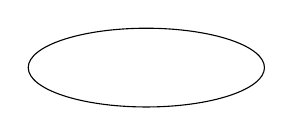
\begin{tikzpicture}
	\draw[scale=0.5] (2,1) ellipse (3cm and 1cm);
\end{tikzpicture}
\end{tcblisting}

圆弧的绘制,我们首先是先确定这条弧起点坐标,然后确定初始初始角的大小,最后的参量是这条圆弧对应的圆的半径大小。

\begin{tcblisting}{tikz lower,listing side text,fonttitle=\bfseries,
	bicolor,colback=xia,colbacklower=tubeijing,colframe=tou,
	righthand width=5cm,title=Arc}

\begin{tikzpicture}
  \draw[orange,very thick,scale=1]
  (3,0) arc (0:75:3cm);
\end{tikzpicture}
\end{tcblisting}

更加清楚的看到是这样的;

\begin{tcblisting}{tikz lower,listing side text,fonttitle=\bfseries,
	bicolor,colback=xia,colbacklower=tubeijing,colframe=tou,
	righthand width=5cm,title=Arc}
\begin{tikzpicture}
  \draw[orange,very thick,scale=1]
  (4,2) arc (0:75:2cm);
  \draw[orange,dashed,scale=1]
  (2,2) circle (2cm);
\end{tikzpicture}
\end{tcblisting}

% 画圆动态图
% \foreach \X in {0,10,...,350}{
% \begin{tikzpicture}
% 	\draw[orange,very thick,scale=1]
%   (3,0) arc (\X:\Y:3cm);
% \end{tikzpicture}
%}

另外,我们还可以绘制虚线的圆、椭圆等,利用在 \verb|\draw[<dashed>]| 设置 <style> 类型。

\begin{tcblisting}{tikz lower,listing side text,fonttitle=\bfseries,
	bicolor,colback=xia,colbacklower=tubeijing,colframe=tou,
	righthand width=5cm,title=Dashed Circle}
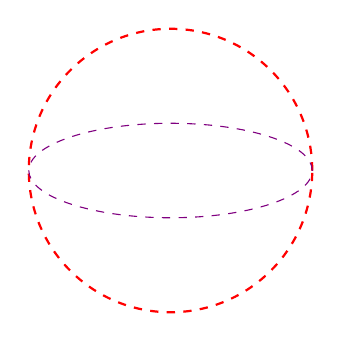
\begin{tikzpicture}
	\draw[red,thick,dashed,scale=0.6]
	 (3,3) circle (3cm);
	 \draw[scale=0.6,dashed,violet] (3,3) ellipse (3cm and 1cm);
\end{tikzpicture}
\end{tcblisting}

\section{TikZ 绘制网格}
\begin{tcolorbox}[enhanced,arc=3mm,boxrule=1.5mm,
	frame hidden,colback=blue!10!white,
	borderline={1mm}{0mm}{blue,dotted} ]
	在很多情况我们利用坐标绘图等会在坐标系中添加网格,网格有助于更加直观和准确的绘制图像,以及更利于读者获取更多信息,在绘图过程中,网格绘制有时候很有必要。绘制网格主要确定两个参量,一个是左下角和右上角的坐标(对角上的坐标),另还可以设置需要的风格。
	\end{tcolorbox}

\begin{tcblisting}{tikz lower,listing side text,fonttitle=\bfseries,
	bicolor,colback=xia,colbacklower=tubeijing,colframe=tou,
	righthand width=5cm,title=Grids}

\begin{tikzpicture}
	\draw[step=1cm,gray,very thin,scale=0.8]
	 (0,0) grid (4,4);
\end{tikzpicture}
\end{tcblisting}

在命令\verb|\begin{tikzpicture}[<xscale>=number1,<yscale>=number2]| 来缩小或者放大所绘制网格的大小比例。或者我们可以同时放大或者缩小;
	
\verb|\begin{tikzpicture}[<scale>=number]|
	

\begin{tcblisting}{tikz lower,listing side text,fonttitle=\bfseries,
	bicolor,colback=xia,colbacklower=tubeijing,colframe=tou,
	righthand width=5cm,title=Grids}
\begin{tikzpicture}
\draw[gray,very thin,scale=0.5]
(0,0) grid (4,4);
\end{tikzpicture}
\end{tcblisting}

\section{颜色填充}

\begin{tcolorbox}[enhanced,arc=3mm,boxrule=1.5mm,
	frame hidden,colback=blue!10!white,
	borderline={1mm}{0mm}{blue,dotted} ]
	在你在我们来选择绘制的网格区域块进行填充,这里我们选择矩形区域块进行填充,在区域块填充过程中,我们可以利用可选参数命令:\verb|\fill[<color>=color]| 是颜色填充命令,命令 \verb|\drawfill[<fill>=color,<draw>=color]| 来进行绘制填充和边缘颜色填充。
	\end{tcolorbox}

下面我们来单独填充绘制的网格区域块;

	\begin{tcblisting}{tikz lower,listing side text,fonttitle=\bfseries,
		bicolor,colback=xia,colbacklower=tubeijing,colframe=tou,
		righthand width=5cm,title=Colour filling}
	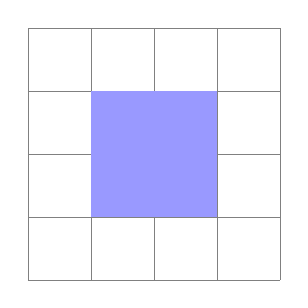
\begin{tikzpicture}
	\draw[gray,very thin,scale=0.8]
	(0,0) grid (4,4);
	\fill[blue!40!white,scale=0.8] (1,1) rectangle (3,3);
	\end{tikzpicture}
	\end{tcblisting}

这里是进行了区域块的颜色填充和边缘颜色的填充;

\begin{tcblisting}{tikz lower,listing side text,fonttitle=\bfseries,
	bicolor,colback=xia,colbacklower=tubeijing,colframe=tou,
	righthand width=5cm,title=Colour filling}
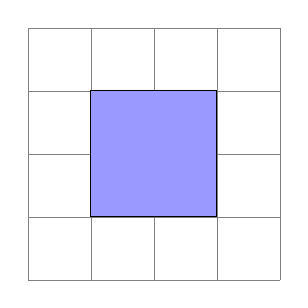
\begin{tikzpicture}
	\draw[gray,very thin,scale=0.8]
	(0,0) grid (4,4);
	\filldraw[fill=blue!40!white, draw=black,scale=0.8]
	 (1,1) rectangle (3,3);
\end{tikzpicture}
\end{tcblisting}

在颜色填充过程中,与上面填充方式不同的是,我们可以通过命令

\verb|\shade[<top color>=color,bottom <color>=color, |

\verb|<left color>=color,<right color>=color]|
但是在现实过程中,当我们设置成:
\begin{lstlisting}
\shade[left color=blue,right color=red,top color=green,bottom color=cyan,scale=0.8] (1,1) rectangle (3,3);
\end{lstlisting}

时,最后结果会只有两个方向的呃颜色显示出来。


\begin{tcblisting}{tikz lower,listing side text,fonttitle=\bfseries,
	bicolor,colback=xia,colbacklower=tubeijing,colframe=tou,
	righthand width=5cm,title=Colour filling}
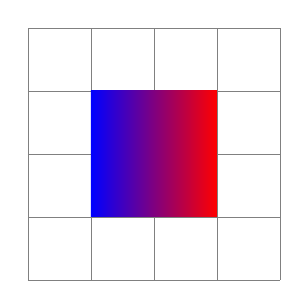
\begin{tikzpicture}
	\draw[gray,very thin,scale=0.8]
	(0,0) grid (4,4);
	\shade[left color=blue,right color=red,scale=0.8] (1,1) rectangle (3,3);
\end{tikzpicture}
\end{tcblisting}

\begin{tcblisting}{tikz lower,listing side text,fonttitle=\bfseries,
	bicolor,colback=xia,colbacklower=tubeijing,colframe=tou,
	righthand width=5cm,title=Colour filling}
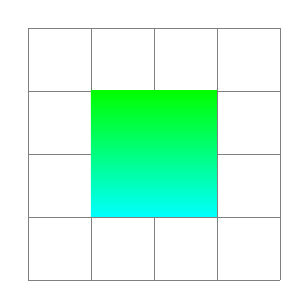
\begin{tikzpicture}
	\draw[gray,very thin,scale=0.8]
	(0,0) grid (4,4);
	\shade[left color=blue,right color=red,top color=green,bottom color=cyan,scale=0.8] (1,1) rectangle (3,3);
\end{tikzpicture}
\end{tcblisting}

我们还可以通过由内而外的颜色填充设置而不是上下或者左右去设置颜色填充。命令

\verb|\shade[<inner color>=color,bottom <outer color>=color]|

下面我们看看效果是这样的
\begin{tcblisting}{tikz lower,listing side text,fonttitle=\bfseries,
	bicolor,colback=xia,colbacklower=tubeijing,colframe=tou,
	righthand width=5cm,title=Colour filling}
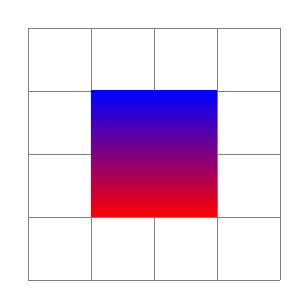
\begin{tikzpicture}
	\draw[gray,very thin,scale=0.8]
	(0,0) grid (4,4);
	\shade[top color=blue,bottom color=red,scale=0.8]
	(1,1) rectangle (3,3);
\end{tikzpicture}
\end{tcblisting}

\begin{tcblisting}{tikz lower,listing side text,fonttitle=\bfseries,
	bicolor,colback=xia,colbacklower=tubeijing,colframe=tou,
	righthand width=5cm,title=Colour filling}
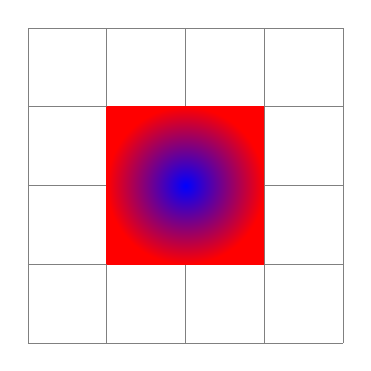
\begin{tikzpicture}
	\draw[gray,very thin,scale=1]
	(0,0) grid (4,4);
	\shade[inner color=blue,outer color=red] (1,1) rectangle (3,3);
\end{tikzpicture}
\end{tcblisting}

最后我们可以通过颜色填充和边缘绘制命令:\verb|\shadedraw| 来进行对内外或者上下左右等方向的填充,

\begin{tcblisting}{tikz lower,listing side text,fonttitle=\bfseries,
	bicolor,colback=xia,colbacklower=tubeijing,colframe=tou,
	righthand width=5cm,title=Colour filling}
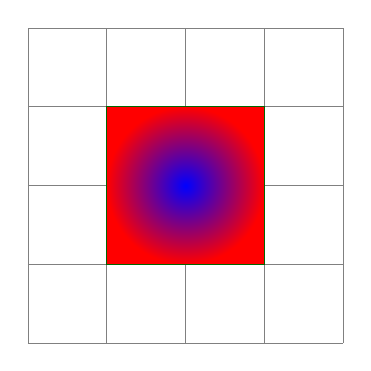
\begin{tikzpicture}
	\draw[gray,very thin,scale=1]
	(0,0) grid (4,4);
	\shade[inner color=blue,outer color=red,draw=black!60!green] (1,1) rectangle (3,3);
\end{tikzpicture}
\end{tcblisting}

\section{直角坐标系的绘制}

平面直角坐标系的绘制主要先确定横坐标以及纵坐标的绘制范围(根据自己绘制图像的需要),然后是取正方向 \verb|\draw[style,->](<x1>,<y1>)--(<x2>,<y2>);|,绘制了 (<x1>,<y1>) 指向 (<x2>,<y2>)的有向线段。在绘制直角坐标系中,我们有时需要对坐标进行刻度绘制,网格辅助等,这节我们来讲述皮昂面直角坐标系的绘制。

首先我们来绘制只有正半轴且无任何标签的平面直角坐标系;

\begin{tcblisting}{tikz lower,listing side text,fonttitle=\bfseries,
	bicolor,colback=xia,colbacklower=tubeijing,colframe=tou,
	righthand width=5cm,title=Axis}
\begin{tikzpicture}
  \draw[thick,->] (0,0) -- (3.5,0);
  \draw[thick,->] (0,0) -- (0,3.5);
\end{tikzpicture}
\end{tcblisting}

\begin{tcolorbox}
	在绘制好坐标和我们需要对坐标轴填上标签:$x$ 轴、$y$ 轴,再添加标签的时候呀我们可以通过命令: \verb|node[<anchor>=west/east/north/south...]| 来固定标签在绘制图像“终点的哪个位置”。
\end{tcolorbox}

\begin{tcblisting}{tikz lower,listing side text,fonttitle=\bfseries,
	bicolor,colback=xia,colbacklower=tubeijing,colframe=tou,
	righthand width=6cm,title=Axis}
\begin{tikzpicture}
\draw[thick,->] (-.5,0) -- (2.5,0)
node[anchor=north west] {x axis};
\draw[thick,->] (0,-.5) -- (0,2.5)
 node[anchor=south east] {y axis};
\end{tikzpicture}
\end{tcblisting}

给坐标系中坐标轴标上刻度是绘制坐标常常做的事情,在表坐标的时候,我们可以一点一点的标,也可以通过 \verb|\foreach| 语句来循环标注;

\begin{tcblisting}{tikz lower,listing side text,fonttitle=\bfseries,
	bicolor,colback=xia,colbacklower=tubeijing,colframe=tou,
	righthand width=6cm,title=Axis}
\begin{tikzpicture}
\draw[thick,->] (0,0) -- (3.5,0)
node[anchor=north west] {x axis};
\draw[thick,->] (0,0) -- (0,3.5)
 node[anchor=south east] {y axis};
 \foreach \x in {0,1,2,3}
   \draw (\x cm,1pt) -- (\x cm,-1pt)
    node[anchor=north] {$\x$};
\foreach \y in {1,2,3}
	\draw (1pt,\y cm) -- (-1pt,\y cm)
	 node[anchor=east] {$\y$};
\end{tikzpicture}
\end{tcblisting}

\begin{tcblisting}{tikz lower,listing side text,fonttitle=\bfseries,
	bicolor,colback=xia,colbacklower=tubeijing,colframe=tou,
	righthand width=6cm,title=Axis}
\begin{tikzpicture} \draw[thick,->] (0,0) -- (3.5,0) node[anchor=north west] {x axis}; \draw[thick,->] (0,0) -- (0,3.5) node[anchor=south east] {y axis}; \foreach \x in {1,2,3} \draw (\x cm,1pt) -- (\x cm,-1pt) node[anchor=north] {$\x$}; \foreach \y in {1,2,3} \draw (1pt,\y cm) -- (-1pt,\y cm) node[anchor=east] {$\y$}; \node[right=2mm,above=.5mm] at (0,0) {O}; \end{tikzpicture}
\end{tcblisting}


\chapter{流程图(程序框图)的绘制}

\section{\emph{tikzstyle} 命令}

这部分我们讲述如何用TikZ宏包进行绘制流程图(简单的程序框图)。程序框图的绘制主要包括以下几个方面:
\begin{itemize}
	\item 宏包调用与 tikzstyle 命令设置
	\item 绘制程序框图中常见的四个框图
	\item 箭头指向连接设置
	\item 某些小细节
\end{itemize}

\textit{导入宏包(导言区)}

\begin{lstlisting}
\usepackage{tikz}  % 绘图宏包
\usetikzlibrary{shapes.geometric, arrows} % 箭头,颜色填充等
\end{lstlisting}

 \begin{tcolorbox}[enhanced,arc=3mm,boxrule=1.5mm,
 	frame hidden,colback=blue!10!white,
 	borderline={1mm}{0mm}{blue,dotted} ]
	在绘制程序框图的过程中,我们首先可以先通过命令: \verb|\tikzstyle|. 来确定绘制程序框图的开始框、输入框、程序框、条件判断框,然后再设置箭头是指向。首先,我们确定一个长度为 3 厘米,高为 1 厘米、内部填充色为 30\% 红色的圆角矩形输入框,其输入设置代码命令如下:
	\end{tcolorbox}

\begin{lstlisting}
\tikzstyle{startstop} = [rectangle, rounded corners,
minimum width=3cm, minimum height=1cm,text centered,
draw=black, fill=red!30]
\end{lstlisting}	

接下来我们来设置输入框,输入框是一个平行四边形,我们在绘制的过程中需要确定对角上的角度大小(可自行改变这个角的大小)设置边缘颜色为黑色而内部填充色为30\% 蓝色,文字设置剧中,宽度为 3 厘米,高度为 1 厘米。

\begin{tcolorbox}
	\verb|\tikzstyle{io}| = [trapezium, trapezium left angle=70, trapezium right angle=110, minimum width=3cm, minimum height=1cm, text centered, draw=black, fill=blue!30]
\end{tcolorbox}

程序框我们是采用矩形 retangle, 利用矩形的绘制和 style 设置进行对程序框的边缘颜色、内部填充颜色以及宽高进行设置。条件框图说起看起来更像一颗钻石,因此,在绘制的过程中我们称之为 diamond,它的设置和前面的相似。

\begin{lstlisting}
\tikzstyle{process} = [rectangle, minimum width=3cm, minimum height=1cm,
text centered, draw=black, fill=orange!30]
\tikzstyle{decision} = [diamond, minimum width=3cm, minimum height=1cm,
 text centered, draw=black, fill=green!30]
\end{lstlisting}
在上面的四个程序框绘制好了以后,我们开始进行链条的设置在导言区需要加入:

\verb|\usetikzlibrary{shapes.geometric, arrows}|

\verb|\tikzstyle{arrow} = [thick,->,>=stealth]|

\section{框图衔接绘制}

在我们进行四个程序框图以及箭头都已经设置好了以后,我们利用箭头开始将前面设置好的框图进行连接起来,
框图之间的链接需要确定两个框图之间的位置关系以及,上下或者左右两个框图之间的距离,在命令 \verb|\begin{tikzpicture}[<style>]| 进行设置。如我们要设置上下左右之间框图距离为 2 厘米,这设置代码如下;

\begin{verbatim}
	\begin{tikzpicture}[node distance=2cm]
		<TikZ code>
		\end{tikzpicture}
\end{verbatim}

To add a node we use the \verb|\node| command. We then add a label for the node in parenthesis. This label is how we refer to the node in the rest of the code. Then in square brackets we add the name of the \verb|\tikzstyle| we want the node to conform to, along with any other formatting options. Then in curly brackets we add the text we want to appear in the block before closing the statement with a semicolon:

\verb|\node (start) [startstop] {Start};|

If we now compile the code you'll see our start block has appeared as expected:

\begin{tcblisting}{tikz lower,listing side text,fonttitle=\bfseries,
	bicolor,colback=xia,colbacklower=tubeijing,colframe=tou,
	righthand width=5cm,title=Colour filling}
\begin{tikzpicture}
\node at (1.5,1){  %   图像绘制的开始
\begin{tikzpicture}[node distance=2cm]
\node (start) [startstop] {Start};
\end{tikzpicture}
                   %   图绘制的结束
};
\end{tikzpicture}

\end{tcblisting}

Now let's add an input block in below the start block. This time we need to tell the node where to position itself. To do this we enter below of followed by an equals sign and a node label into the square brackets. We could also use above of, right of or left of if we wanted the block to appear somewhere else. We'll tell it to position itself below the start block:
\begin{verbatim}
	\node (in1) [io, below of=start] {Input};
\end{verbatim}

\begin{tcblisting}{tikz lower,listing side text,fonttitle=\bfseries,
	bicolor,colback=xia,colbacklower=tubeijing,colframe=tou,
	righthand width=5cm,title=Start}
\node at (2,1){   %   图像绘制的开始
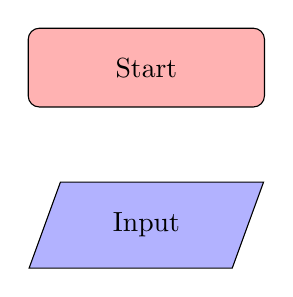
\begin{tikzpicture}[node distance=2cm]
\node (start) [startstop] {Start};
\node (in1) [io, below of=start] {Input};
\end{tikzpicture} %   图绘制的结束		
};
\end{tcblisting}

Now lets add in a process block and a decision block.

\begin{verbatim}
\node (pro1) [process, below of=in1] {Process 1};
\node (dec1) [decision, below of=pro1] {Decision 1};
\end{verbatim}

If we compile the code you'll notice that the gap between the green decision block and the orange process block isn't as big as the other gaps:

\begin{tcblisting}{tikz lower,listing side text,fonttitle=\bfseries,
	bicolor,colback=xia,colbacklower=tubeijing,colframe=tou,
	righthand width=5cm,title=Input}
\node at (2,1){   %    图像绘制的开始	
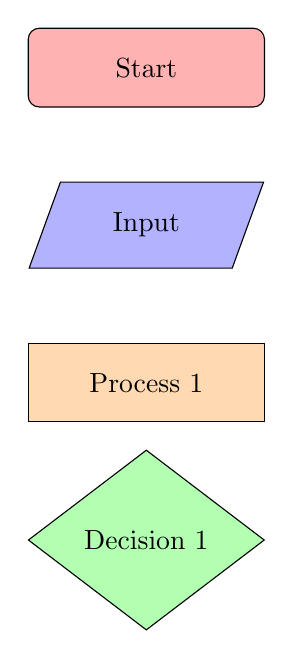
\begin{tikzpicture}[node distance=2cm]
\node (start) [startstop] {Start};
\node (in1) [io, below of=start] {Input};
\node (pro1) [process, below of=in1] {Process 1};
\node (dec1) [decision, below of=pro1] {Decision 1};
\end{tikzpicture} %    图绘制的结束		
};
\end{tcblisting}

This is because the decision block, being a diamond, is taller than the other blocks. Therefore we can manually adjust its position using the yshift variable. If we enter yshift=-0.5cm it will move the decision block vertically down by 0.5cm which should make the gap more regular:

\begin{tcblisting}{tikz lower,listing side text,fonttitle=\bfseries,
	bicolor,colback=xia,colbacklower=tubeijing,colframe=tou,
	righthand width=5cm,title=Process 1}
\node at (2,1){    %   图像绘制的开始	
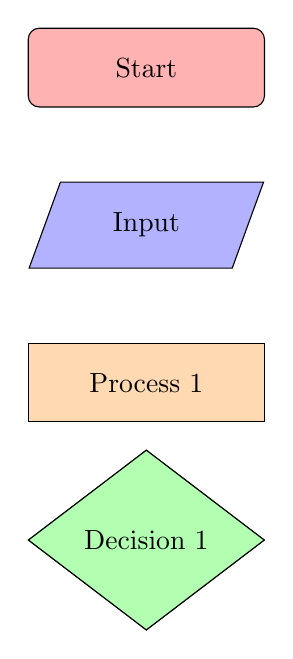
\begin{tikzpicture}[node distance=2cm]
\node (start) [startstop] {Start};
\node (in1) [io, below of=start] {Input};
\node (pro1) [process, below of=in1] {Process 1};
\node (dec1) [decision, below of=pro1] {Decision 1};
\node (dec1) [decision, below of=pro1] {Decision 1};
\end{tikzpicture}	%   图绘制的结束		
 };
\end{tcblisting}

Now lets add in two process blocks coming out of the decision block, one below it and one to the right of it. Again, we'll need to alter the positioning using yshift for the block below and xshift for the block to the right. Let's finish off adding the blocks by adding in an output block and a stop block.

\begin{minipage}{0.5\linewidth}
	\begin{lstlisting}
		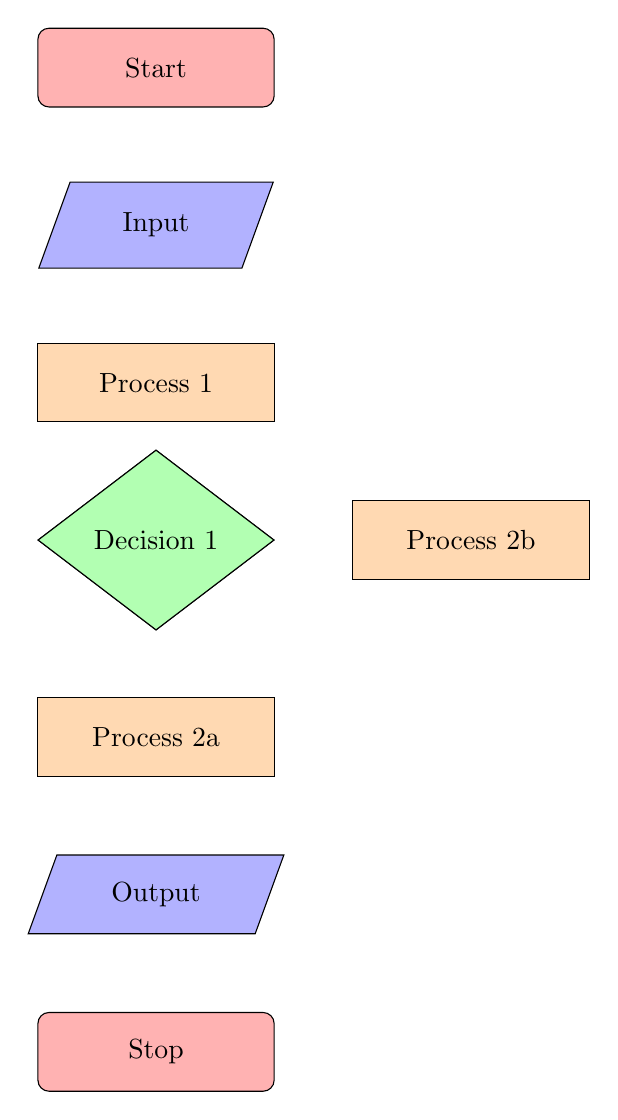
\begin{tikzpicture}[node distance=2cm]
			\node (start) [startstop] {Start};
			\node (in1) [io, below of=start] {Input};
			\node (pro1) [process, below of=in1] {Process 1};
			\node (dec1) [decision, below of=pro1] {Decision 1};
			\node (dec1) [decision, below of=pro1] {Decision 1};
		\node (pro2a) [process, below of=dec1, yshift=-0.5cm] {Process 2a};
		\node (pro2b) [process, right of=dec1, xshift=2cm] {Process 2b};
		\node (out1) [io, below of=pro2a] {Output};
		\node (stop) [startstop, below of=out1] {Stop};
		\end{tikzpicture}		
	\end{lstlisting}
\end{minipage}\quad
\begin{minipage}{0.45\linewidth}
	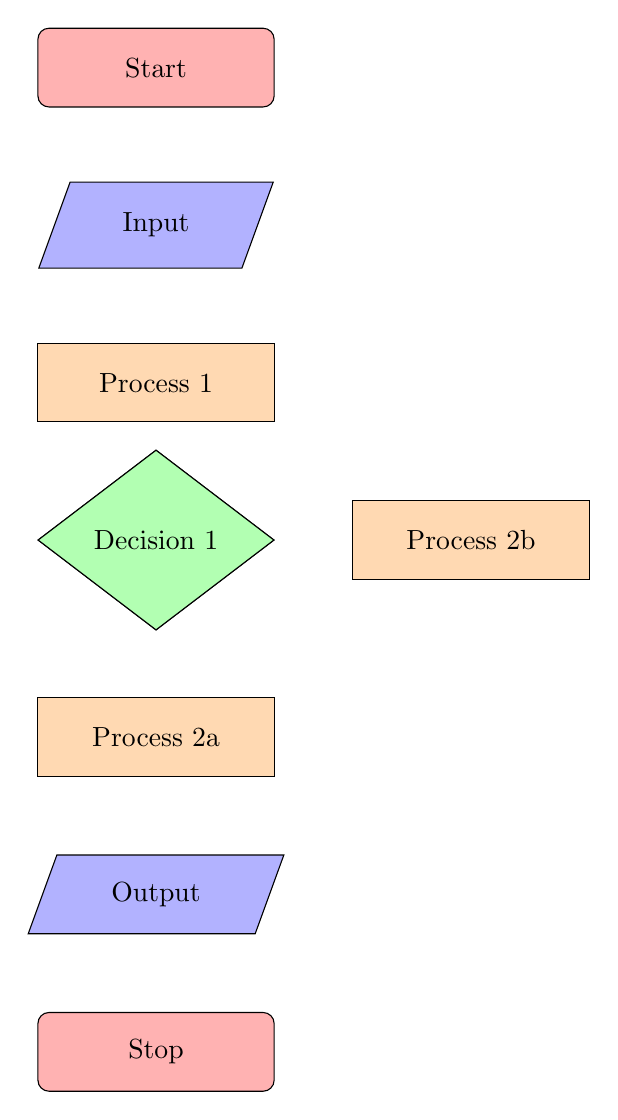
\begin{tikzpicture}[node distance=2cm]
	\node (start) [startstop] {Start};
	\node (in1) [io, below of=start] {Input};
	\node (pro1) [process, below of=in1] {Process 1};
	\node (dec1) [decision, below of=pro1] {Decision 1};
	\node (dec1) [decision, below of=pro1] {Decision 1};
\node (pro2a) [process, below of=dec1, yshift=-0.5cm] {Process 2a};
\node (pro2b) [process, right of=dec1, xshift=2cm] {Process 2b};
\node (out1) [io, below of=pro2a] {Output};
\node (stop) [startstop, below of=out1] {Stop};
\end{tikzpicture}
\end{minipage}


\section{箭头的绘制}

To finish off our flowchart we need to add the arrows in. To draw an arrow we use the \verb|\draw| command and then specify the tikzstyle we prepared for arrows using square brackets. We then enter the label of the node we want the arrow to start from, followed by two dashes and then the label corresponding to the node we want the arrow to terminate at. The labels need to be in parenthesis and we need to make sure we close the statement with a semicolon. Lets add arrows in between the start block and the input block, the input and process 1, process 1 and decision 1, decision 1 and process 2a and between decision 1 and process 2b:
\begin{lstlisting}
\draw [arrow] (start) -- (in1);
\draw [arrow] (in1) -- (pro1);
\draw [arrow] (pro1) -- (dec1);
\draw [arrow] (dec1) -- (pro2a);
\draw [arrow] (dec1) -- (pro2b);
\end{lstlisting}


\begin{tcblisting}{tikz lower,listing side text,fonttitle=\bfseries,
	bicolor,colback=xia,colbacklower=tubeijing,colframe=tou,
	righthand width=5.5cm,title=Decision 1}
\node at (2,1) {   % 绘图的开始
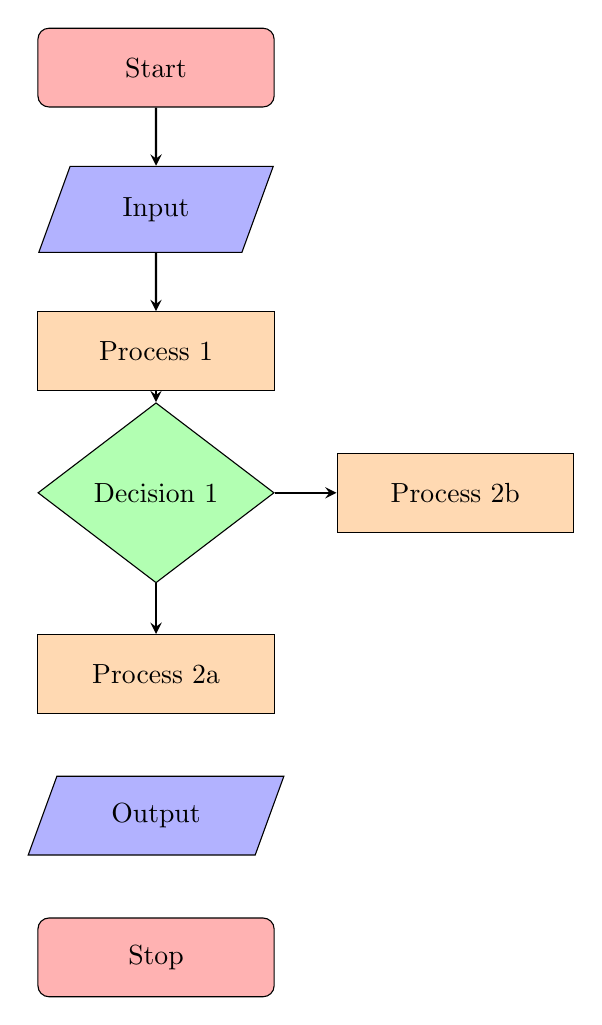
\begin{tikzpicture}[node distance=1.8cm]
\node (start) [startstop] {Start};
\node (in1) [io, below of=start] {Input};
\node (pro1) [process, below of=in1] {Process 1};
\node (dec1) [decision, below of=pro1] {Decision 1};
\node (pro2a) [process, below of=dec1, yshift=-0.5cm] {Process 2a};
\node (pro2b) [process, right of=dec1, xshift=2cm] {Process 2b};
\node (out1) [io, below of=pro2a] {Output};
\node (stop) [startstop, below of=out1] {Stop};
\draw [arrow] (start) -- (in1);
\draw [arrow] (in1) -- (pro1);
\draw [arrow] (pro1) -- (dec1);
\draw [arrow] (dec1) -- (pro2a);
\draw [arrow] (dec1) -- (pro2b);
\end{tikzpicture} % 绘图的结束
};
\end{tcblisting}


\begin{tcolorbox}
	As we have arrows coming out of a decision block we need to add some text to these two arrows. To do this we use more nodes, however this time we don't need to use the \verb|\node| command, we just type the word node in after the two dashes and then the text in curly brackets:
	\begin{lstlisting}
	\draw [arrow] (dec1) -- node {yes} (pro2a);
    \draw [arrow] (dec1) -- node {no} (pro2b);
	\end{lstlisting}
	\begin{tikzpicture}[node distance=2cm]
		\node (dec1) [decision, below of=pro1] {Decision 1};
        \node (pro2a) [process, below of=dec1, yshift=-0.5cm] {Process 2a};
        \node (pro2b) [process, right of=dec1, xshift=2cm] {Process 2b};
		\draw [arrow] (dec1) -- node {yes} (pro2a);
       \draw [arrow] (dec1) -- node {no} (pro2b);
	\end{tikzpicture}
\end{tcolorbox}

\emph{If we now compile the code you'll see the text has been added but not in a very helpful place:}

\begin{tcolorbox}
	To fix this we specify which of the node's anchors \emph{TikZ} should use to fix the nodes to the lines. To do this we use square brackets immediately after the keyword node and then enter anchor= followed by the anchor. For the yes node we'll use the east anchor and for the no node we'll use the south anchor:
\begin{lstlisting}
\draw [arrow] (dec1) -- node[anchor=east] {yes} (pro2a);
\draw [arrow] (dec1) -- node[anchor=south] {no} (pro2b);
\end{lstlisting}
\begin{tikzpicture}[node distance=2cm]
\node (dec1) [decision, below of=pro1] {Decision 1};
 \node (pro2a) [process, below of=dec1, yshift=-0.5cm] {Process 2a};
 \node (pro2b) [process, right of=dec1, xshift=2cm] {Process 2b};
\draw [arrow] (dec1) -- node[anchor=east] {yes} (pro2a);
\draw [arrow] (dec1) -- node[anchor=south] {no} (pro2b);
	\end{tikzpicture}
\end{tcolorbox}

Now let's draw the final arrows in:

\begin{lstlisting}
\draw [arrow] (pro2b) -- (pro1);
\draw [arrow] (pro2a) -- (out1);
\draw [arrow] (out1) -- (stop);	
\end{lstlisting}

\begin{tcblisting}{tikz lower,listing side text,fonttitle=\bfseries,
	bicolor,colback=xia,colbacklower=tubeijing,colframe=tou,
	righthand width=5.5cm,title=Colour filling}
\node at (2,1) {   % 绘图的开始
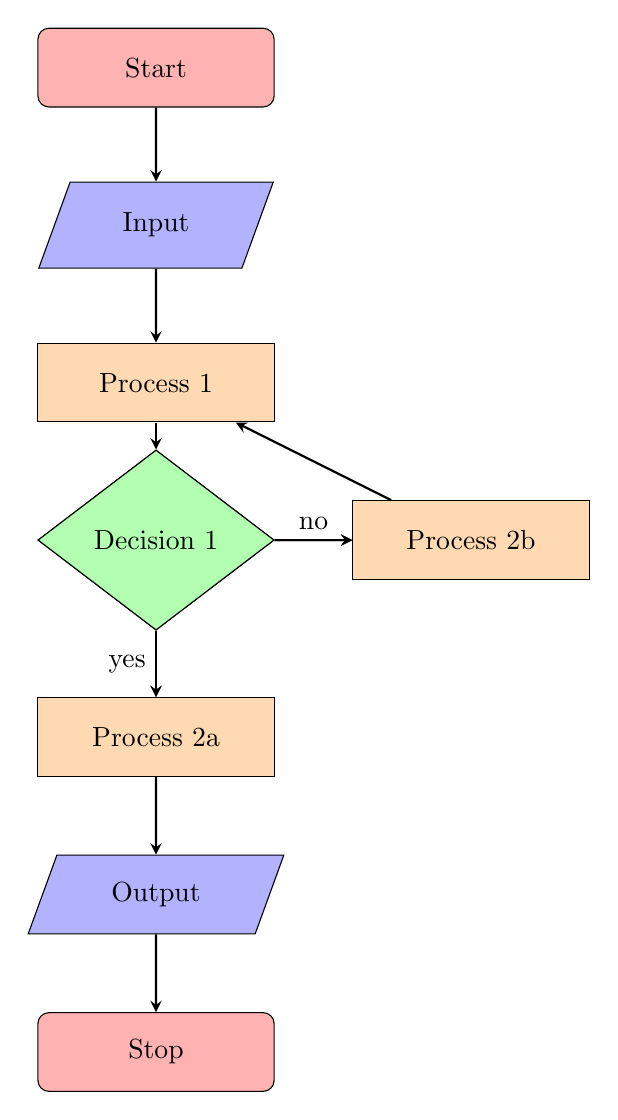
\begin{tikzpicture}[node distance=2cm,scale=0.6]
\node (start) [startstop] {Start};
\node (in1) [io, below of=start] {Input};
\node (pro1) [process, below of=in1] {Process 1};
\node (dec1) [decision, below of=pro1] {Decision 1};
\node (pro2a) [process, below of=dec1, yshift=-0.5cm] {Process 2a};
\node (pro2b) [process, right of=dec1, xshift=2cm] {Process 2b};
\node (out1) [io, below of=pro2a] {Output};
\node (stop) [startstop, below of=out1] {Stop};
\draw [arrow] (start) -- (in1);
\draw [arrow] (in1) -- (pro1);
\draw [arrow] (pro1) -- (dec1);
\draw [arrow] (dec1) -- (pro2a);
\draw [arrow] (dec1) -- (pro2b);
\node (dec1) [decision, below of=pro1] {Decision 1};
\node (pro2a) [process, below of=dec1, yshift=-0.5cm] {Process 2a};
\node (pro2b) [process, right of=dec1, xshift=2cm] {Process 2b};
\draw [arrow] (dec1) -- node[anchor=east] {yes} (pro2a);
\draw [arrow] (dec1) -- node[anchor=south] {no} (pro2b);
\draw [arrow] (pro2b) -- (pro1);
\draw [arrow] (pro2a) -- (out1);
\draw [arrow] (out1) -- (stop);
\end{tikzpicture} % 绘图结束
};
\end{tcblisting}

\begin{tcolorbox}
	You'll also notice that the arrow from process 2b to process 1 is diagonal and therefore doesn't look right. To improve this we can swap the first dash for a bar symbol which will make the arrow go in a vertical direction before going in a horizontal direction:

	\verb|\draw [arrow] (pro2b) |- (pro1);|

\begin{minipage}{0.48\linewidth}
	\begin{tikzpicture}[node distance=2cm,scale=0.4]
		\node (pro1) [process, below of=in1] {Process 1};
		\node (dec1) [decision, below of=pro1] {Decision 1};
		 \node (pro2a) [process, below of=dec1, yshift=-0.5cm] {Process 2a};
		 \node (pro2b) [process, right of=dec1, xshift=2cm] {Process 2b};
		\draw [arrow] (dec1) -- node[anchor=east] {yes} (pro2a);
		\draw [arrow] (dec1) -- node[anchor=south] {no} (pro2b);
		\draw [arrow] (pro2b) -- (pro1);
			\end{tikzpicture}
\end{minipage}\quad
\begin{minipage}{0.48\linewidth}
	\begin{tikzpicture}[node distance=2cm,scale=0.4]
		\node (pro1) [process, below of=in1] {Process 1};
		\node (dec1) [decision, below of=pro1] {Decision 1};
		 \node (pro2a) [process, below of=dec1, yshift=-0.5cm] {Process 2a};
		 \node (pro2b) [process, right of=dec1, xshift=2cm] {Process 2b};
		\draw [arrow] (dec1) -- node[anchor=east] {yes} (pro2a);
		\draw [arrow] (dec1) -- node[anchor=south] {no} (pro2b);
		\draw [arrow] (pro2b) |- (pro1);
			\end{tikzpicture}
\end{minipage}
\end{tcolorbox}
		
\section{框内文字内容宽度设置}

The final thing we should discuss is the text width. At the moment all our text fits nicely inside our shapes. However, if for example, we add some more text to process 2a, you'll see the shape just extends horizontally until the text fits:
\begin{lstlisting}
	\node (pro2a) [process, below of=dec1, yshift=-0.5cm] {Process 2a text text text text text text text text text text};
\end{lstlisting}

\begin{tikzpicture}
	\node (pro2a) [process, below of=dec1, yshift=-0.5cm] {Process 2a text text text text text text text text text text};
\end{tikzpicture}

This now becomes a bit messy. To improve it we can specify the text width for these nodes by entering text width= followed by a length into our \verb|\tikzstyles|:

\begin{lstlisting}
	\tikzstyle{process} = [rectangle, minimum width=3cm, minimum height=1cm, text centered, text width=3cm, draw=black, fill=orange!30]
\end{lstlisting}
		
\begin{tikzpicture}
	\tikzstyle{process} = [rectangle, minimum width=3cm, minimum height=1cm, text centered, text width=3cm, draw=black, fill=orange!30]
\end{tikzpicture}



\chapter{CircuiTikZ 绘制电路图}

\section{CircuiTikZ 基本命令}
这部分我们讲解用  TikZ 来绘制一个简单的电路图,主要用到的宏包: \verb|\usepackage{circuitikz}|。关于 circuitikz 更多的内容学习可以查看 circuitikz 宏包说明,这里的讲解主要起到一个抛砖引玉的作用。下面我们从以下几个方面进行内容的学习:
\begin{itemize}
  \item circuitikz 宏包以及基本命令
  \item 简单电路图的绘制
  \item 电路图常见电路图元件
\end{itemize}


\begin{tcolorbox}
	We don't need to load the TikZ package as well because it automatically gets loaded with circuitikz. To draw a diagram we use the circuitikz environment. We then fill the environment with a single \verb|\draw| command ending in a semicolon.
\end{tcolorbox}

\begin{lstlisting}
\begin{circuitikz}
draw<circuitikz code>;
\end{circuitikz}
\end{lstlisting}

\section{Circuitikz 绘制简单电路图}

The general format is then a pair of co-ordinates followed by a link and then the next pair of co-ordinates. You can then keep adding further links and co-ordinates like a chain. The link could simply be a line which is achieved using two dashes, or it could be an electrical component. To add a component on a line we use the keyword to followed by square brackets containing the name of the component. For example, we'll start at (0,0) and head towards (0,4) adding a battery in. We'll then add an ammeter in on the way to (4,4) followed by a simple line to (4,0). We'll complete the circuit by adding a lamp in on the way back (0,0):

This is what the diagram looks like compiled:

\begin{minipage}{0.48\linewidth}
	\begin{lstlisting}
		\begin{circuitikz}
			\draw(0,0) to[battery] (0,4)
			to[ammeter] (4,4) -- (4,0)
			to[lamp] (0,0);
		\end{circuitikz}
	\end{lstlisting}
\end{minipage}\quad
\begin{minipage}{0.48\linewidth}
\begin{circuitikz}
\draw(0,0) to[battery] (0,4)
	to[ammeter] (4,4) -- (4,0)
	to[lamp] (0,0);
\end{circuitikz}
\end{minipage}

Now let's add a voltmeter in parallel to the lamp. To do this we want to branch off the bottom line part way along, then drop down, insert the meter, and then join back up with the bottom line before its end:

\begin{tcolorbox}
	

	\begin{minipage}{0.48\linewidth}
		\begin{lstlisting}
			\begin{circuitikz}
			   \draw(0,0) to[battery]
			   (0,4) to[ammeter]
			   (4,4) -- (4,0)
			   to[lamp] (0,0)
			   (0.5,0) -- (0.5,-2)
			   to[voltmeter]
			   (3.5,-2) -- (3.5,0);
			\end{circuitikz}
			\end{lstlisting}
	\end{minipage}\quad
	\begin{minipage}{0.48\linewidth}
		\begin{circuitikz}
			\draw(0,0) to[battery]
			(0,4) to[ammeter]
			(4,4) -- (4,0)
			to[lamp] (0,0)
			(0.5,0) -- (0.5,-2)
			to[voltmeter]
			(3.5,-2) -- (3.5,0);
		 \end{circuitikz}
	\end{minipage}

	

\end{tcolorbox}

If we wanted to make the points where the lines join into proper terminals represented by circles, we could add *-* into the square brackets where we added the lamp in. This will add terminals in at the co-ordinates either side of the component. Therefore we need to shorten the lines either side of the lamp so that the terminals appear at our line joins, and then we need to fill in the gaps:

\begin{tcolorbox}
	\begin{minipage}{0.48\linewidth}
		\begin{lstlisting}
			\begin{circuitikz}
			\draw(0,0) to[battery] (0,4)
			to[ammeter] (4,4) -- (4,0) -- (3.5,0)
			to[lamp, *-*] (0.5,0) -- (0,0)
			(0.5,0) -- (0.5,-2)
			to[voltmeter] (3.5,-2) -- (3.5,0);
			\end{circuitikz}
			\end{lstlisting}
	\end{minipage}\quad
	\begin{minipage}{0.48\linewidth}
		\begin{circuitikz}
			\draw(0,0) to[battery]
			(0,4) to[ammeter]
			(4,4) -- (4,0)
			to[lamp] (0,0)
			(0.5,0) -- (0.5,-2)
			to[voltmeter]
			(3.5,-2) -- (3.5,0);
		 \end{circuitikz}
	\end{minipage}
\end{tcolorbox}

Next we'll add a capacitor in between the lamp and ammeter. We specify a capacitor with a capital C:

\begin{tcolorbox}
	\begin{minipage}{0.48\linewidth}
		\begin{lstlisting}
			\begin{circuitikz} \draw
				(0,0) to[battery] (0,4)
				  to[ammeter] (4,4)
				  to[C] (4,0) -- (3.5,0)
				  to[lamp, *-*] (0.5,0) -- (0,0)
				(0.5,0) -- (0.5,-2)
				  to[voltmeter] (3.5,-2) -- (3.5,0);
				\end{circuitikz}
			\end{lstlisting}
	\end{minipage}\quad
	\begin{minipage}{0.48\linewidth}
		\begin{circuitikz} \draw
			(0,0) to[battery] (0,4)
			  to[ammeter] (4,4)
			  to[C] (4,0) -- (3.5,0)
			  to[lamp, *-*] (0.5,0) -- (0,0)
			(0.5,0) -- (0.5,-2)
			  to[voltmeter] (3.5,-2) -- (3.5,0);
			\end{circuitikz}
	\end{minipage}
\end{tcolorbox}

Often we'll want to add labels to our diagrams to give the reader more information. To be able to include electrical units in our labels we need to add the siunitx option into the \verb|\usepackage| command:
\verb|\usepackage[siunitx]{circuitikz}|

We could add a label to the ammeter like this:

\verb|to[ammeter, l=2<\ampere>]|

\begin{minipage}{0.48\linewidth}
	\begin{lstlisting}
		\begin{circuitikz}
			\draw(0,0) to[battery] (0,4)
			  to[ammeter, l=2<\ampere>] (4,4)
			  to[C] (4,0) -- (3.5,0)
			  to[lamp, *-*] (0.5,0) -- (0,0)
			(0.5,0) -- (0.5,-2)
			  to[voltmeter] (3.5,-2) -- (3.5,0);
			\end{circuitikz}
		\end{lstlisting}
\end{minipage}\quad
\begin{minipage}{0.48\linewidth}
	\begin{circuitikz} \draw
		(0,0) to[battery] (0,4)
		  to[ammeter, l=2<\ampere>] (4,4)
		  to[C] (4,0) -- (3.5,0)
		  to[lamp, *-*] (0.5,0) -- (0,0)
		(0.5,0) -- (0.5,-2)
		  to[voltmeter] (3.5,-2) -- (3.5,0);
		\end{circuitikz}
\end{minipage}

The l tells \LaTeX{} we are adding a label. Notice that we put the unit commands in pointed brackets. As we're using SI units we could add an SI prefix in. We could also move the label to below the symbol by adding underscore immediately after the l:

\verb|to[ammeter, l_=2<\milli\ampere>]|

\begin{minipage}{0.48\linewidth}
	\begin{lstlisting}
		\begin{circuitikz}
			\draw(0,0) to[battery] (0,4)
			  to[ammeter, l_=2<\milli\ampere>] (4,4)
			  to[C] (4,0) -- (3.5,0)
			  to[lamp, *-*] (0.5,0) -- (0,0)
			(0.5,0) -- (0.5,-2)
			  to[voltmeter] (3.5,-2) -- (3.5,0);
			\end{circuitikz}
		\end{lstlisting}
\end{minipage}\quad
\begin{minipage}{0.48\linewidth}
	\begin{circuitikz} \draw
		(0,0) to[battery] (0,4)
		  to[ammeter, l_=2<\milli\ampere>] (4,4)
		  to[C] (4,0) -- (3.5,0)
		  to[lamp, *-*] (0.5,0) -- (0,0)
		(0.5,0) -- (0.5,-2)
		  to[voltmeter] (3.5,-2) -- (3.5,0);
		\end{circuitikz}
\end{minipage}

As we are displaying current we could place the label next to an arrow on the line by changing the l to an i:

\verb|to[ammeter, i_=2<\milli\ampere>]|

\begin{tcolorbox}
\begin{minipage}{0.48\linewidth}
	\begin{lstlisting}
		\begin{circuitikz}
			\draw(0,0) to[battery] (0,4)
			to[ammeter, i_=2<\milli\ampere>] (4,4)
			  to[C] (4,0) -- (3.5,0)
			  to[lamp, *-*] (0.5,0) -- (0,0)
			(0.5,0) -- (0.5,-2)
			  to[voltmeter] (3.5,-2) -- (3.5,0);
			\end{circuitikz}
		\end{lstlisting}
\end{minipage}\quad
\begin{minipage}{0.48\linewidth}
	\begin{circuitikz} \draw
		(0,0) to[battery] (0,4)
		to[ammeter, i_=2<\milli\ampere>] (4,4)
		  to[C] (4,0) -- (3.5,0)
		  to[lamp, *-*] (0.5,0) -- (0,0)
		(0.5,0) -- (0.5,-2)
		  to[voltmeter] (3.5,-2) -- (3.5,0);
		\end{circuitikz}
\end{minipage}
\end{tcolorbox}

Let's add some labels in next to the capacitor and the voltmeter. With the capacitor we can just begin the label with an equals following the capital C:

\begin{circuitikz} \draw
	(0,0) to[battery] (0,4)
	  to[ammeter, i_=2<\milli\ampere>] (4,4)
	  to[C=3<\farad>] (4,0) -- (3.5,0)
	  to[lamp, *-*] (0.5,0) -- (0,0)
	(0.5,0) -- (0.5,-2)
	  to[voltmeter, l=3<\kilo\volt>] (3.5,-2) -- (3.5,0)
	;
	\end{circuitikz}

\emph{We could also change the colour of a component like this:}

\verb|to[voltmeter, l=3<\kilo\volt>, color=red]|
	
	\begin{circuitikz}
		\draw(0,0) to[battery] (0,4)
		  to[ammeter, i_=2<\milli\ampere>] (4,4)
		  to[C=3<\farad>] (4,0) -- (3.5,0)
		  to[lamp, *-*] (0.5,0) -- (0,0)
		(0.5,0) -- (0.5,-2)
		to[voltmeter, l=3<\kilo\volt>, color=red]
		 (3.5,-2) -- (3.5,0)
		;
		\end{circuitikz}
	
\section{Circuitikz 常见的电路元件}
		Notice that the components stay the same size but the spacing between everything changes.

\emph{Let's finish this post by looking at a selection of other components we could use:}

\begin{tcolorbox}
	\begin{minipage}{0.48\linewidth}
		\begin{lstlisting}
			\begin{circuitikz}
				\draw
				(0,0) to[R, o-o] (2,0)
				(4,0) to[vR, o-o] (6,0)
				(0,2) to[transmission line, o-o] (2,2)
				(4,2) to[closing switch, o-o] (6,2)
				(0,4) to[european current source, o-o] (2,4)
				(4,4) to[european voltage source, o-o] (6,4)
				(0,6) to[empty diode, o-o] (2,6)
				(4,6) to[full led, o-o] (6,6)
				(0,8) to[generic, o-o] (2,8)
				(4,8) to[sinusoidal voltage source, o-o] (6,8)
				;
				\end{circuitikz}
			\end{lstlisting}
	\end{minipage}\quad
	\begin{minipage}{0.48\linewidth}
		\begin{circuitikz}
			\draw
			(0,0) to[R, o-o] (2,0)
			(4,0) to[vR, o-o] (6,0)
			(0,2) to[transmission line, o-o] (2,2)
			(4,2) to[closing switch, o-o] (6,2)
			(0,4) to[european current source, o-o] (2,4)
			(4,4) to[european voltage source, o-o] (6,4)
			(0,6) to[empty diode, o-o] (2,6)
			(4,6) to[full led, o-o] (6,6)
			(0,8) to[generic, o-o] (2,8)
			(4,8) to[sinusoidal voltage source, o-o] (6,8)
			;
			\end{circuitikz}
	\end{minipage}
	\end{tcolorbox}

	From the bottom left we have; a resistor, a variable resistor, a transmission line, a closing switch, a european current source, a european voltage source, an empty diode, a full led, a generic bipole and a sinusoidal voltage source.

	\begin{tcolorbox}[enhanced,arc=3mm,boxrule=1.5mm,
		frame hidden,colback=blue!10!white,
		borderline={1mm}{0mm}{blue,dotted} ]
		Bipoles aren't the only type of component we can use. We can also add in monopoles, tripoles, double bipoles, logic gates and amplifiers. However we can't use the to keyword to add these in as we've done before, because they don't naturally fit on a single line. Instead we use node notation. For example, this is how we would display an antenna:
		\end{tcolorbox}

		\verb|(0,0) node[antenna] {}|
		

		You can add text to the symbol using the curly brackets, but note that we still need to enter curly brackets even if we don't want to use them.
		
		Here are some more command examples:

\begin{lstlisting}
   (4,0) node[pmos] {}
   (0,4) node[op amp] {}
   (4,4) node[american or port] {}
   (0,8) node[transformer] {}
   (4,8) node[spdt] {}
\end{lstlisting}


\chapter{从 Geogebra 中获取绘制图像的 \LaTeX{} 代码}

In this video we're going to look at using GeoGebra to generate TikZ code to use in our LaTeX documents. GeoGebra is a great tool for creating and displaying mathematical diagrams. You can get a copy of GeoGebra from the GeoGebra website, \emph{www.geogebra.org.}

\DeclareTotalTColorBox{\diabox}{ O{} v m }
{ bicolor,nobeforeafter,equal height group=diabox,width=14cm,
fonttitle=\bfseries\ttfamily,adjusted title={#2},center title,
colframe=blue!20!black,leftupper=0mm,rightupper=0mm,colback=black!75!white,#1}
{ \tikz\path[fill zoom image={#2}] (0,0) rectangle (\linewidth,10cm);%
\tcblower#3}
\diabox{Tikzfig1.png}{用  Polygon 绘制圆}

Next we'll add a polygon inside our circle using the Polygon tool:

\diabox{Tikzfig2.png}{在绘制的圆中通过绘图工具 Angle tool 绘制角}

Then we'll measure an angle inside this polygon using the Angle tool:

\diabox{Tikzfig3.png}{}

Now we'll add a straight line going through two points on the circle using the Line through Two Points tool:

\diabox{Tikzfig4.png}{}

We'll finish up by turning the grid on. To do this we select the Move tool, right click on the background and select the Grid option:

\diabox{Tikzfig5.png}{}

Now to export this as TikZ code we open the file menu, hover over Export and click on Graphics View as PGF/TikZ:

\centerline{\includegraphics[scale=0.55]{Tikzfig6}}

We then tell GeoGebra how much of the grid we want included in our tikzpicture by altering the x and y minimum and maximum points. You'll see a blue box represent this area on the grid. Next we check the format is set to \LaTeX article class and then click the generate button:

\diabox{Tikzfig7.png}{}

Now if we hit Copy to Clipboard we can then paste it into an empty tex file. You'll notice that it has generated a preamble where it loads up the tikz package and a TikZ library, it sets the page style to empty and it also defines a new command:

\begin{lstlisting}
\usepackage{pgf,tikz}
\usetikzlibrary{arrows}
\pagestyle{empty}
\newcommand{\degre}{\ensuremath{^\circ}}
\end{lstlisting}

Then it begins the document and defines some colours before opening a tikzpicture environment:

\begin{lstlisting}
\definecolor{qqwuqq}{rgb}{0,0.39,0}
\definecolor{zzttqq}{rgb}{0.6,0.2,0}
\definecolor{xdxdff}{rgb}{0.49,0.49,1}
\definecolor{qqqqff}{rgb}{0,0,1}
\definecolor{cqcqcq}{rgb}{0.75,0.75,0.75}
\end{lstlisting}

If we compile the code we'll see it appear in the document. As it's generated
from TikZ code rather than an image, it's very high quality:

\diabox{Tikzfig8.png}{}

We could also turn the TikZ picture into a figure to give us more control over things like positioning. To do this we simply enclose the tikzpicture environment in the figure environment. We can then add a placement specifier, a caption and a label:

\begin{lstlisting}
	\begin{figure}[!h]
		<tikzpicture environment>
		\label{circle1}
		\caption{TikZ from GeoGebra}
	\end{figure}
\end{lstlisting}

Now if we want to include this figure in an existing document we can copy over everything in the figure environment. We also need to make sure we copy over the relevant parts of the preamble if they're not in our existing docs preamble already. Therefore we'll copy over the \verb|\usepackage| command and \verb|\usetikzlibrary| command as well as the \verb|\newcommand| definition. Finally we also need to copy over the colour definitions.

If we go back to GeoGebra we can alter the way our diagram looks by right clicking on it and changing the object properties. For example we can change colours, point styles, line styles and line thickness.

\diabox{Tikzfig9.png}{}

Another useful thing we can do with GoeGebra is export to Tikz in a beamer format so that we can add diagrams into presentations. To do this we export like before except we select the LaTeX (beamer class) option:

\centerline{\includegraphics[scale=1]{Tikzfig10.png}}




\centerline{\includegraphics[scale=0.5]{geogebra1.png}}



\centerline{\includegraphics[scale=0.5]{geogebra2.png}}






%\nocite{*}
%\begin{thebibliography}{99}
%	
%	
%\end{thebibliography}


\end{document}

